% !TeX spellcheck = en_US
\section{Multidimensional Linear Interpolation}

\subsection{Theory}

One of the easiest ways to interpolate a new value between two known values is linear interpolation. It takes the closest values and creates a linear function between them.

In one dimension linear interpolation is pretty trivial. For example, let's assume that we have 20 random points $P$ between 0 and 1 (\textcolor{Red}{\textbullet} and  \textcolor{Blue}{\textbullet} in Figure \ref{fig:one-dim-interpolation}) and have a new point $I$ (\textcolor{Green}{\textbullet}) at $0.4$ for which we want to interpolate. Finding the two closest points \textcolor{Red}{\textbullet} above and below is trivial as there is only one dimension to compare. Now, if we have measured a value $f(P)$ for each of these points, a straight line (\textcolor{LightGreen}{\textbf{|}}) between the two closest values can be drawn and an interpolated value for $f(I)$ can be found. 

\begin{figure}[h] % TODO: h is temporary 
	\centering
	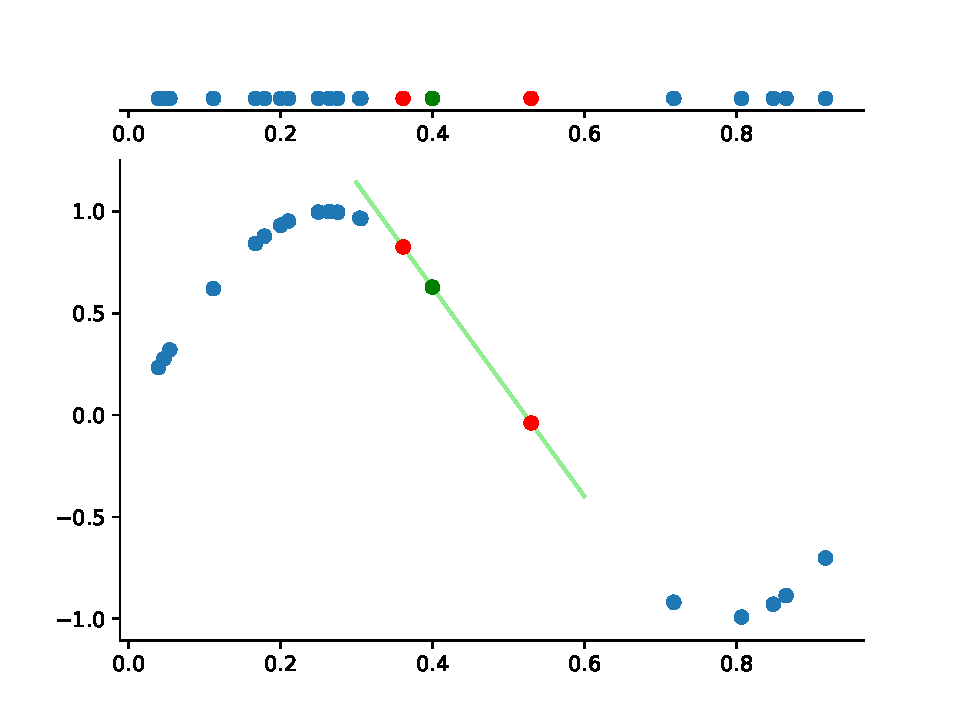
\includegraphics[width=0.8\linewidth]{images/vis1d.pdf}
	\caption{one-dimensional example of linear interpolation}
	\label{fig:one-dim-interpolation}
\end{figure}

In two dimensions things get more complicated as we now have a set of points with $X$ and $Y$ coordinates (Figure \ref{fig:3dinterpolate-1}). One fast way to find the closest points to the point that should be interpolated is using Delaunay triangulation. This separates the space between the points into triangles while trying to maximize their smallest angle. Afterwards the closest three points can be found very quickly by checking the nodes of the surrounding triangle  (Figure \ref{fig:3dinterpolate-2}). If we now again have a function $f(X,Y)$ similar to the one-dimensional example (Figure \ref{fig:3dinterpolate-3}), we can create a unique plain through the three points and get the interpolated value for any $X$ and $Y$ on this layer.


\begin{figure}[h] % also temporary
	\centering
	\begin{subfigure}[t]{0.5\textwidth}
		\centering
		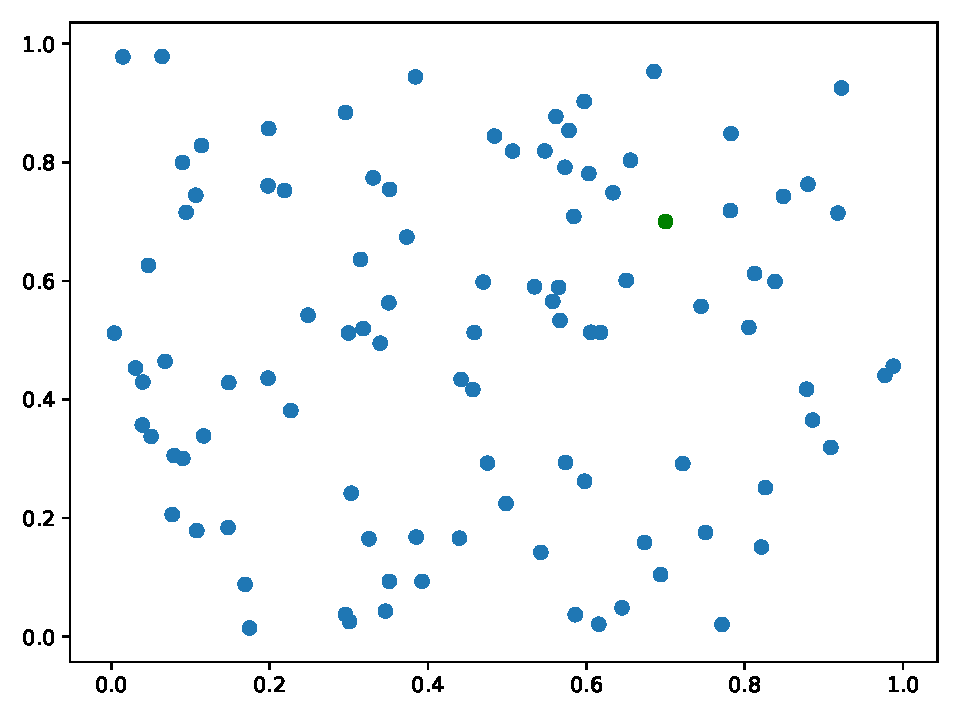
\includegraphics[width=\linewidth]{images/vis2d1.pdf}
		\caption{Lorem ipsum}
	\label{fig:3dinterpolate-1}
	\end{subfigure}%
	~ 
	\begin{subfigure}[t]{0.5\textwidth}
		\centering
		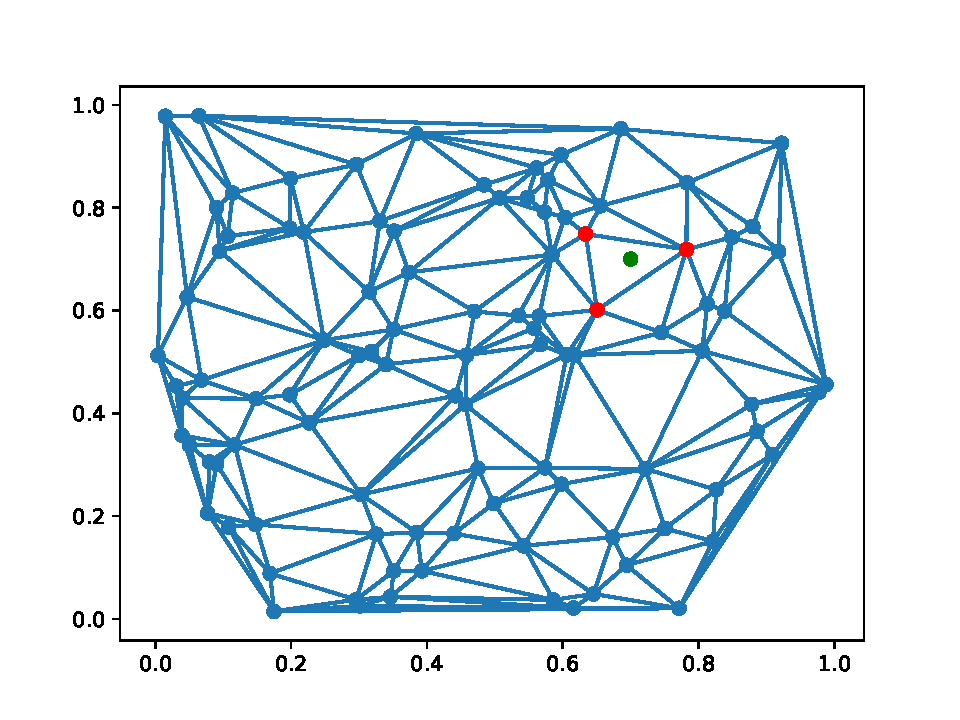
\includegraphics[width=\linewidth]{images/vis2d2.pdf}
		\caption{Lorem ipsum, lorem ipsum,Lorem ipsum, lorem ipsum,Lorem ipsum}
		\label{fig:3dinterpolate-2}
	\end{subfigure}
	\caption{Caption place holder}

\end{figure}

\begin{figure}[h] % TODO: h is temporary 
	\centering
	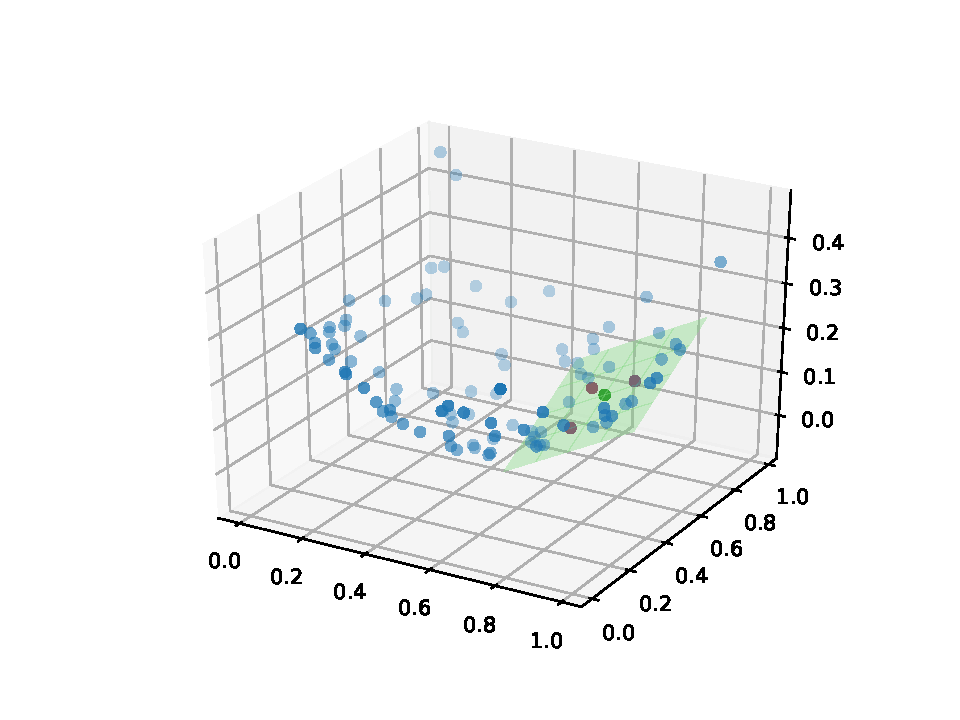
\includegraphics[width=0.8\linewidth]{images/vis2d3.pdf}
	\caption{two-dimensional example of linear interpolation}
	\label{fig:3dinterpolate-3}
\end{figure}

This approach has the advantage that it can be extended in more than two dimensions by replacing the triangle in the Delaunay triangulation with an n-simplex in n dimensions. The \texttt{scipy.spatial.Delaunay} python function allows to quickly calculate it thanks to the \texttt{Qhull} library\footnote{\url{http://www.qhull.org/}}. One noticeable limitation of this method is that data can't be extrapolated. Therefore the possible output is limited to the convex hull of the input parameter space (as seen in Figure \ref{fig:3dinterpolate-2}).

\subsection{Implementation}
\label{sec:griddata-implementation}
For doing the actual interpolations, the \texttt{scipy.interpolate.griddata} function is used with the \texttt{method="linear"} argument which itself uses \texttt{scipy.interpolate.LinearNDInterpolator} to do the interpolation as described above. The function is given a $6\times n$ matrix of the six parameters and an $n$-sized list of the water retention fraction for those $n$ simulations. In addition, \texttt{griddata} supports not only calculating interpolations for one set of parameters, but also for lists of parameters which allows to quickly generate 2d diagrams as seen in \ref{the_chapter_where_I_show_the_v_alpha_plots}.

\subsection{Results}